\section{问题及解决方案}
记录实验过程中所遇到的问题以及解决方法.

\subsection{高分影像参数问题}
ENVI5.3 ``open as'' 中可自动读取GF-1影像. 但是辐射校正需要的绝对定标系数, 如图~\ref{fig:0201}为空, 无法自动更新. 

\begin{figure}[htbp]
    \centering
    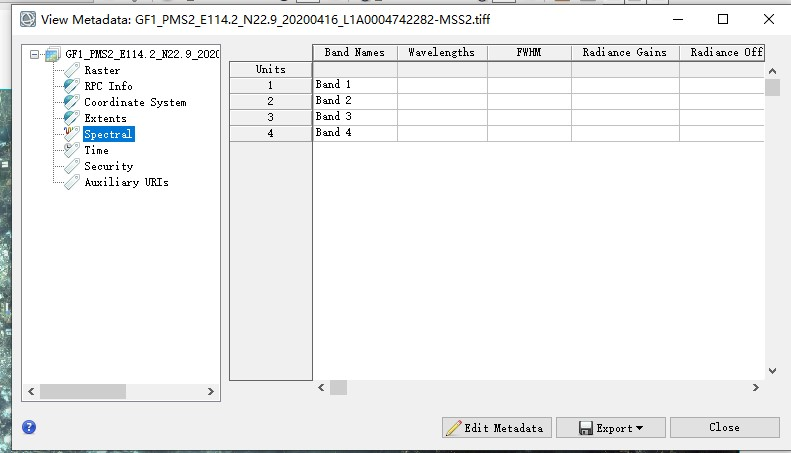
\includegraphics[height=12em]{pic/q1_05.jpg}
    \caption{高分影像参数}
    \label{fig:0201}
\end{figure}

此时需要安装~\href{http://blog.sina.com.cn/s/blog_764b1e9d0102xjbj.html#cmt_5AD807AE-3B2A6BFD-6A4E9A6B-91B-8EF}{ENVI扩展工具: 中国国产卫星支持工具}~, 通过插件打开高分一号卫星数据, 弹出警告如图~\ref{fig:0202}所示:

\begin{figure}[htbp]
    \centering
    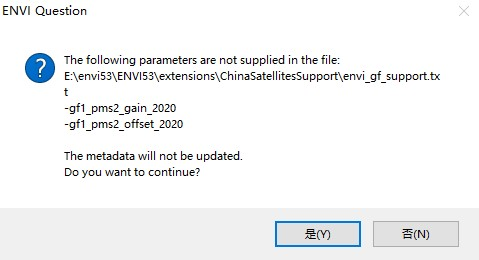
\includegraphics[height=12em]{pic/q1_01.jpg}
    \caption{影像读取警告}
    \label{fig:0202}
\end{figure}

选择``是'', 继续操作, 此时通过右键``View Metadata'', 发现报错如图~\ref{fig:0203}所示, 同时进行辐射定标操作时, 弹出错误:
\begin{itemize}
    \item ``Calibration requires gain and offset for each band''
\end{itemize}

\begin{figure}[!htbp]
    \centering
    \subfloat[]{\label{fig:0203a}
    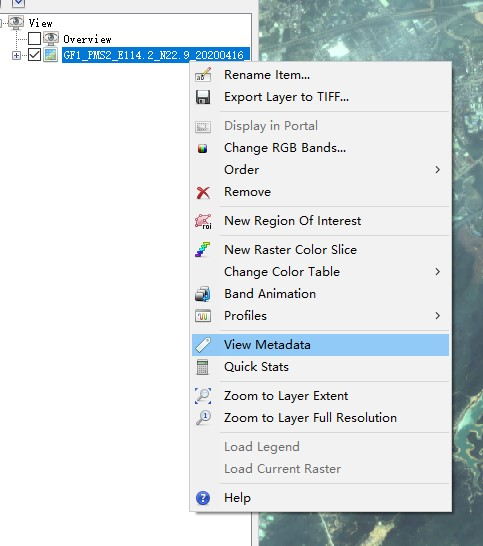
\includegraphics[height=12em]{pic/q1_02.jpg}}
    \qquad
    \subfloat[]{\label{fig:0203b}
    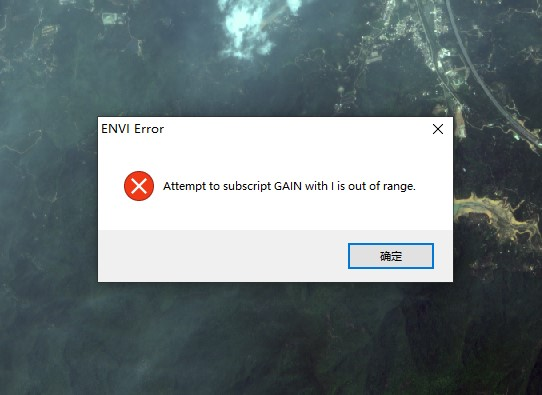
\includegraphics[height=12em]{pic/q1_04.jpg}}
    \\[12pt]
    \subfloat[辐射定标参数]{\label{fig:0203c}
    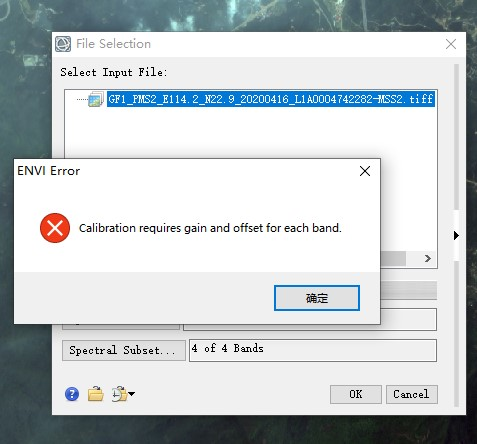
\includegraphics[height=12em]{pic/q1_03.jpg}}
    \caption{元数据报错与辐射定标报错}
    \label{fig:0203}
\end{figure}

虽通过中国卫星支持工具打开, 但影像的 ``gain'' 和 ``offset''参数并未正确读入. 根据~\ref{fig:0202}提示, 两个参数在插件的参数文件中未被支持, 分别为:
\begin{itemize}
    \item ``-gf1\_pms2\_gain\_2020''
    \item ``-gf1\_pms2\_offset\_2020''
\end{itemize}

查看插件文件参数, 如图~\ref{fig:0204a}所示, 最新数据只有2019年, 的确不存在图~\ref{fig:0202}所示两个2020年参数.

\begin{figure}[htbp]
    \centering
    \subfloat[插件参数]{\label{fig:0204a}
    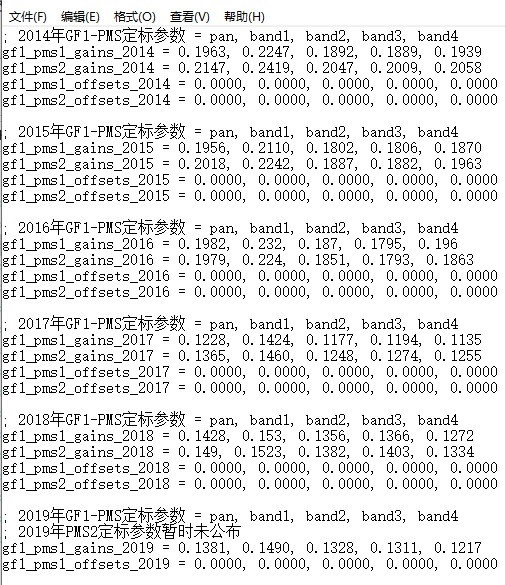
\includegraphics[height=15em]{pic/q1_06.jpg}}
    \qquad
    \subfloat[中心参数]{\label{fig:0204b}
    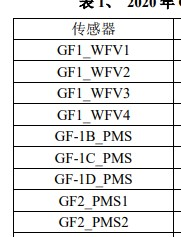
\includegraphics[width=10em]{pic/q1_07.jpg}}
    \caption{插件参数文件与提供参数}
    \label{fig:0204}
\end{figure}

需要在~\href{http://www.cresda.com/CN/Downloads/dbcs/index.shtml}{中国资源卫星应用中心}~中查询. 其结果如图~\ref{fig:0204b}, 中国资源卫星应用中心所提供数据也不包含GF1-PMS1与GF1-PMS2在2020年的数据.

因此可理解为, 其使用参数并未变化, 使用2018和2019年高分一号的PMS1和PMS2参数来代替2020年参数. 获取影像 ``gain'' 与 ``offset'' 参数后, 便可进行高分影像的预处理实验. 

\subsection{正射校正后影像变色}
在对高分一号数据进行预处理最后一步正射校正时, 发现影像出现变色, 如图~\ref{fig:0205}所示. 

\begin{figure}[htbp]
    \centering
    \subfloat[]{\label{fig:0205a}
    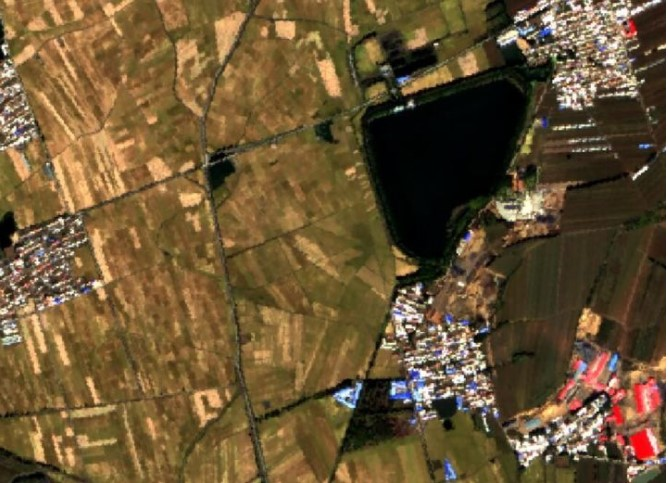
\includegraphics[width=12em]{pic/q2_01.jpg}}
    \qquad
    \subfloat[]{\label{fig:0205b}
    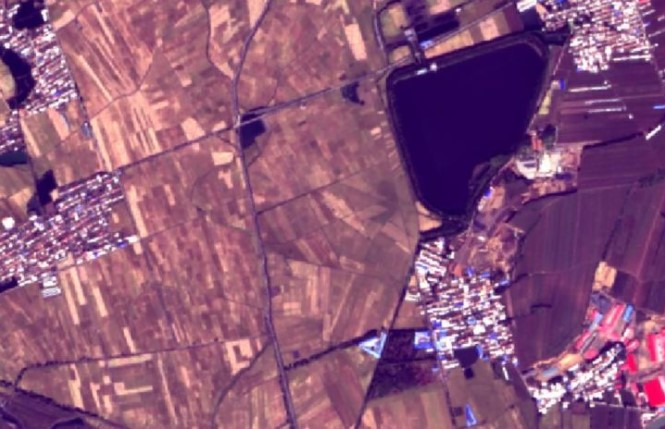
\includegraphics[width=12em]{pic/q2_02.jpg}}
    \caption{正射校正前后影像对比}
    \label{fig:0205}
\end{figure}

解决方法是, 通过 ``Edit Header File'' 工具, 添加 ``Ignore Data Value'', 如图\ref{fig:0206a}, 并设其为 ``0'', 如图\ref{fig:0206b}所示, 即可得到正常的影像.

\begin{figure}[htbp]
    \centering
    \subfloat[]{\label{fig:0206a}
    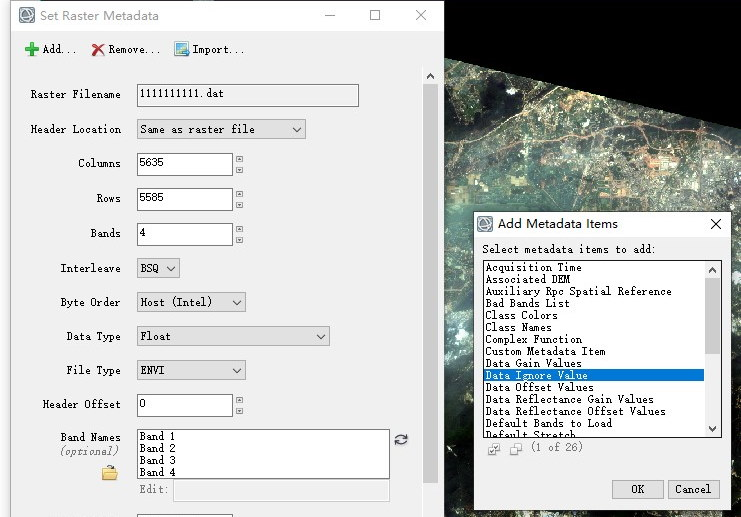
\includegraphics[width=15em]{pic/q2_03.jpg}}
    \qquad
    \subfloat[]{\label{fig:0206b}
    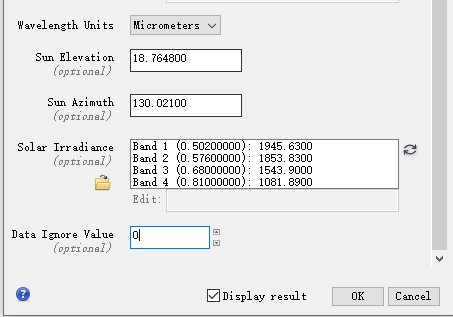
\includegraphics[width=15em]{pic/q2_04.jpg}}
    \caption{忽略无效值}
    \label{fig:0206}
\end{figure}

\subsection{ENVI打开哨兵影像}
直接通过欧空局软件SNAP ``Save As'' 操作会弹出报错, 如图~\ref{fig:0207}所示. 其原因是ENVI要求所有波段影像分辨率相同, 而Sentinel-2影像不同波段分辨率不同, 如Band2其分辨率为10m X 10m, 而Band4分辨率为20m X 20m.

\begin{figure}[!htbp]
    \centering
    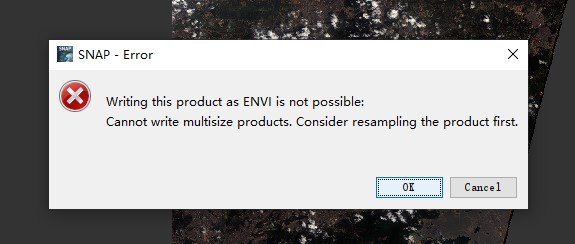
\includegraphics[height=12em]{pic/q3_01.jpg}
    \caption{SNAP另存报错}
    \label{fig:0207}
\end{figure}

因此需要对原始哨兵影像进行10m x 10m的重采样, 如图~\ref{fig:0208a}所示, 再进行 ``Save As'' 操作, 其结果如图~\ref{fig:0208b}所示, 所得到的是波段拆分结果. 

\begin{figure}[!htbp]
    \centering
    \subfloat[操作]{\label{fig:0208a}
    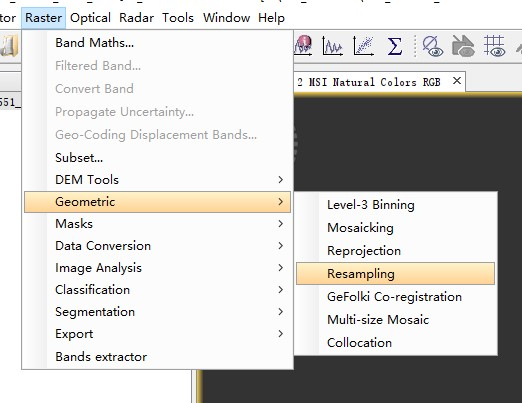
\includegraphics[width=0.7\textwidth]{pic/q3_02.jpg}}
    \\[12pt]
    \subfloat[结果]{\label{fig:0208b}
    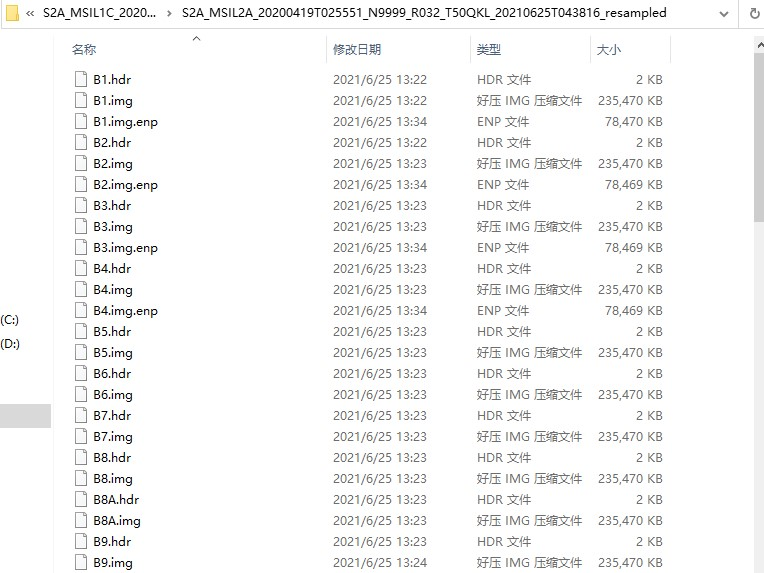
\includegraphics[width=0.7\textwidth]{pic/q3_03.jpg}}
    \caption{SNAP重采样结果}
    \label{fig:0208}
\end{figure}

之后在ENVI中打开B2, B3, B4三个波段, 使用 ``Layer Stacking'' 进行波段合成, 其过程如图~\ref{fig:0209}所示, 便可在ENVI中操作Sentinel-2影像.

\begin{figure}[!htbp]
    \centering
    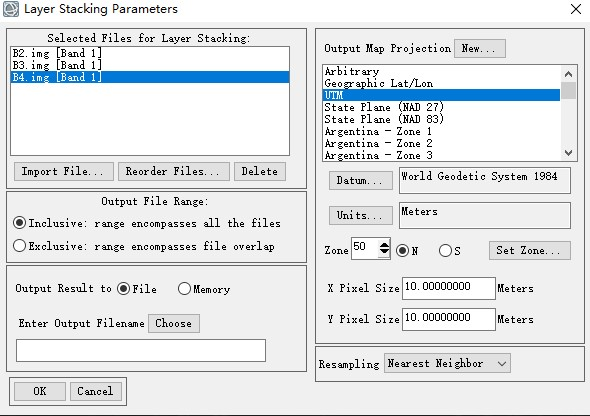
\includegraphics[height=15em]{pic/q3_04.jpg}
    \caption{ENVI波段叠加}
    \label{fig:0209}
\end{figure}

\subsection{不同源影像配准}
至此, GF-1影像与Sentinel-2影像预处理完毕, 此时发现同一地物在两张影像中位置不同, 存在一定偏差, 如图~\ref{fig:0210}所示, 左图~\ref{fig:0210a}为GF-1影像, 右图~\ref{fig:0210b}为S2影像. 十字红线交叉点代表同一经纬度地物, 可明显发现, GF-1影像中对应浅蓝色厂房角点在S2影像中向左有偏移, 因此需要对两幅影像做精细匹配.

\begin{figure}[!htbp]
    \centering
    \subfloat[GF-1]{\label{fig:0210a}
    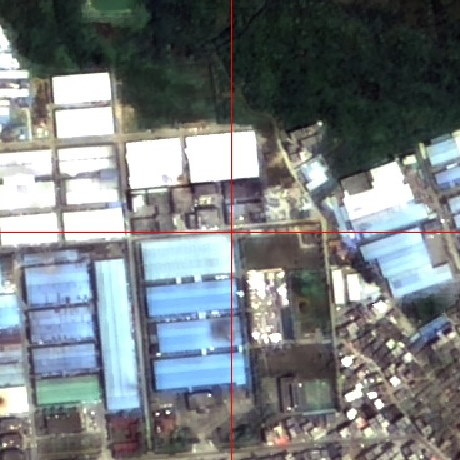
\includegraphics[height=13em]{pic/q4_01.jpg}}
    \qquad
    \subfloat[S2]{\label{fig:0210b}
    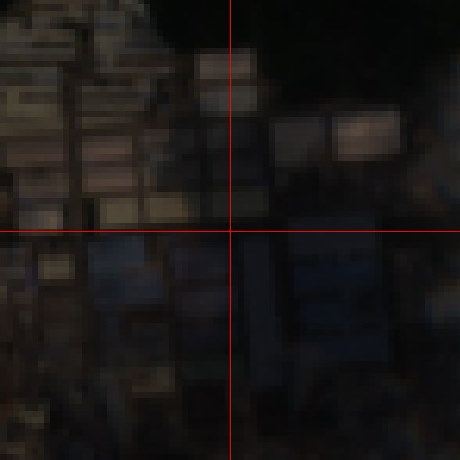
\includegraphics[height=13em]{pic/q4_02.jpg}}
    \caption{不同源影像同一地物}
    \label{fig:0210}
\end{figure}

使用ENVi的 ``Image Registration'' 工具进行影像精细匹配. 以GF-1影像作为基准影像, S2影像作为待配准影像, 手动勾选同名点, 如图~\ref{fig:0211}所示, 左图~\ref{fig:0211a}中粉色点为GF-1影像勾选同名点, 右图~\ref{fig:0211b}中绿色点为S2影像勾选同名点, 数字代表对应序号.

\begin{figure}[!htbp]
    \centering
    \subfloat[GF-1]{\label{fig:0211a}
    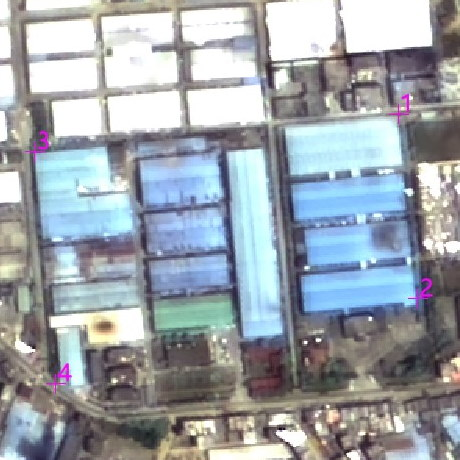
\includegraphics[width=15em]{pic/q4_04.jpg}}
    \qquad
    \subfloat[S2]{\label{fig:0211b}
    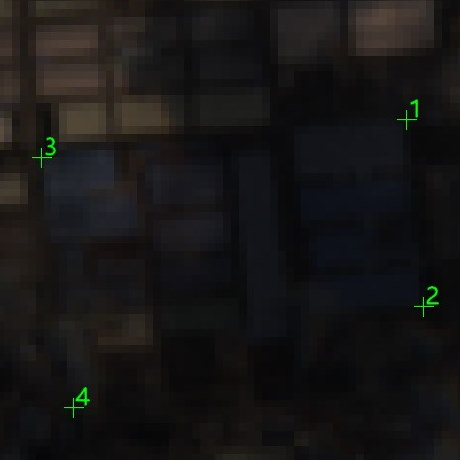
\includegraphics[width=15em]{pic/q4_05.jpg}}
    \caption{精细匹配同名点标定}
    \label{fig:0211}
\end{figure}

ENVI要求至少9对同名点才可进行影像匹配, 手动标了30对同名点, 使其均匀分布在GF-1影像与S2影像重叠部分, 进行精细配准. 以上为手动标同名点方法. 也可以使用ENVI中自带的同名点标定工具, 如图~\ref{fig:0212}所示.

\begin{figure}[!htbp]
    \centering
    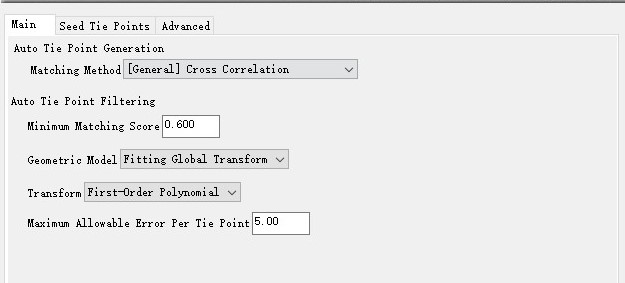
\includegraphics[height=12em]{pic/q4_03.jpg}
    \caption{自动标定同名点工具}
    \label{fig:0212}
\end{figure}

其中关键参数含义如下:
\begin{description}
    \item[Minimum Matching Score] 匹配分数, 越高同名点匹配精度越高
    \item[Maximum Allowable Error Per Tie Point] 每对同名点允许的误差, 越低同名点匹配精度越高 
\end{description}

通过对上述两个参数的限制, 如将 ``Minimum Matching Score'' 设置为 ``0.8'', 将 ``Maximum Allowable Error Per Tie Point'' 设置为 ``1.0'', 可得到较为准确的同名点对, 之后进行影像精匹配, 同名点寻找结果如图~\ref{fig:0213}所示:

\begin{figure}[!htbp]
    \centering
    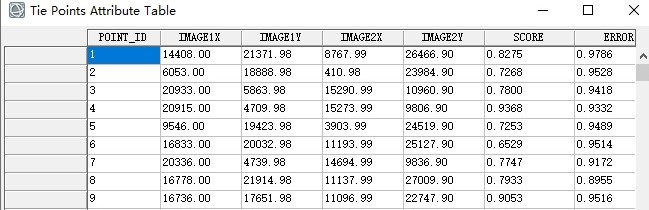
\includegraphics[height=10em]{pic/q4_08.jpg}
    \caption{自动标定同名点结果}
    \label{fig:0213}
\end{figure}

\begin{figure}[!htbp]
    \centering
    \subfloat[GF-1]{\label{fig:0214a}
    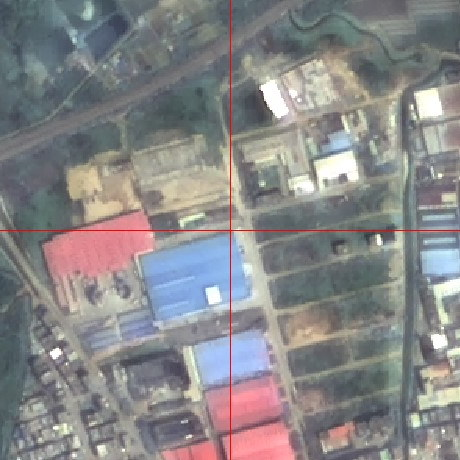
\includegraphics[width=15em]{pic/q4_06.jpg}}
    \qquad
    \subfloat[S2]{\label{fig:0214b}
    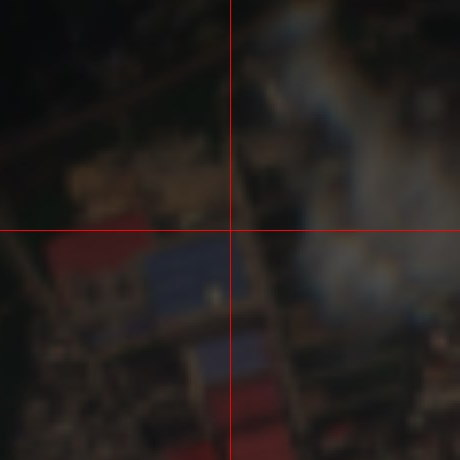
\includegraphics[width=15em]{pic/q4_07.jpg}}
    \caption{影像精匹配结果}
    \label{fig:0214}
\end{figure}

其结果如上图~\ref{fig:0214}所示, 十字红线交叉点代表同一经纬度地物, GF-1影像与S2影像中十字红线皆为厂房交点, 经过多次目视判别, 同一地物在两幅图像经纬度一致, 认为匹配精度可以接受. 

\subsection{不同源影像色彩不同}
超分影像要求低分辨率影像和高分辨率影像色调一致, 不能一明一暗. 因此需要通过直方图匹配的方式将S2影像色调调整至与GF-1相似. 使用\href{http://blog.sina.com.cn/s/blog_764b1e9d0102vqws.html}{ENVI扩展工具:直方图匹配工具}, 遇到报错如图~\ref{fig:0215}所示: 

\begin{figure}[!htbp]
    \centering
    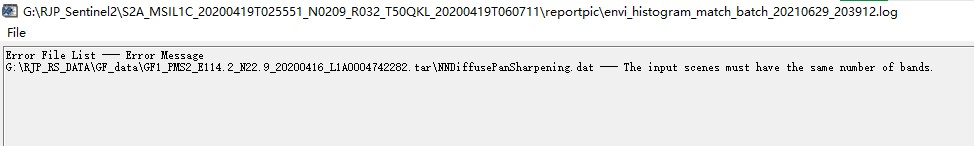
\includegraphics[height=5em]{pic/q5_01.jpg}
    \caption{报错一: 波段数量}
    \label{fig:0215}
\end{figure}

其报错为波段数目不同, 因此将GF-1四个波段通过波段拆分, 再将RGB三个波段进行合成, 得到与S2相同波段数的图像. 又遇到问题, 如图~\ref{fig:0216}所示, 现在还在想问题解决方法. 

\begin{figure}[!htbp]
    \centering
    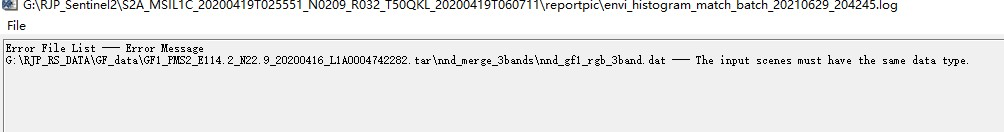
\includegraphics[height=4em]{pic/q5_02.jpg}
    \caption{报错二: 数据类型}
    \label{fig:0216}
\end{figure}

猜想是否因为无效数据的原因, 目前已尝试裁剪相同小块图像进行直方图匹配, 仍然报错. 

\subsection{融合结果}
发现GF-1光学影像与融合结果可以直接用来做超分影像数据集. 其色调完全一致也不存在定位误差.

\begin{figure}[!htbp]
    \centering
    \subfloat[融合前光学影像]{\label{fig:0217a}
    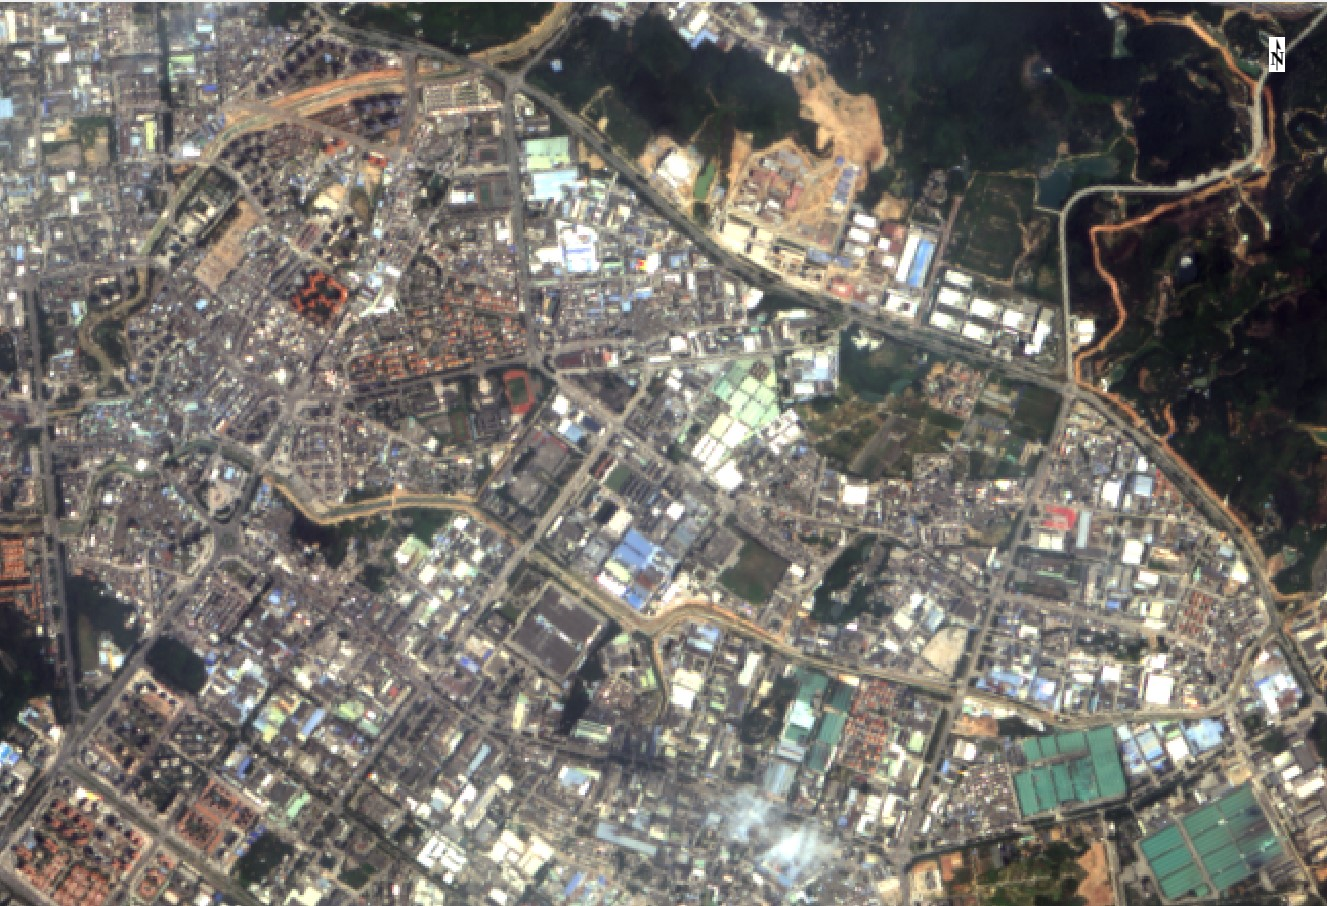
\includegraphics[height=20em]{pic/res01_01.jpg}}
    \\[12pt]
    \subfloat[融合后光学影像]{\label{fig:0217b}
    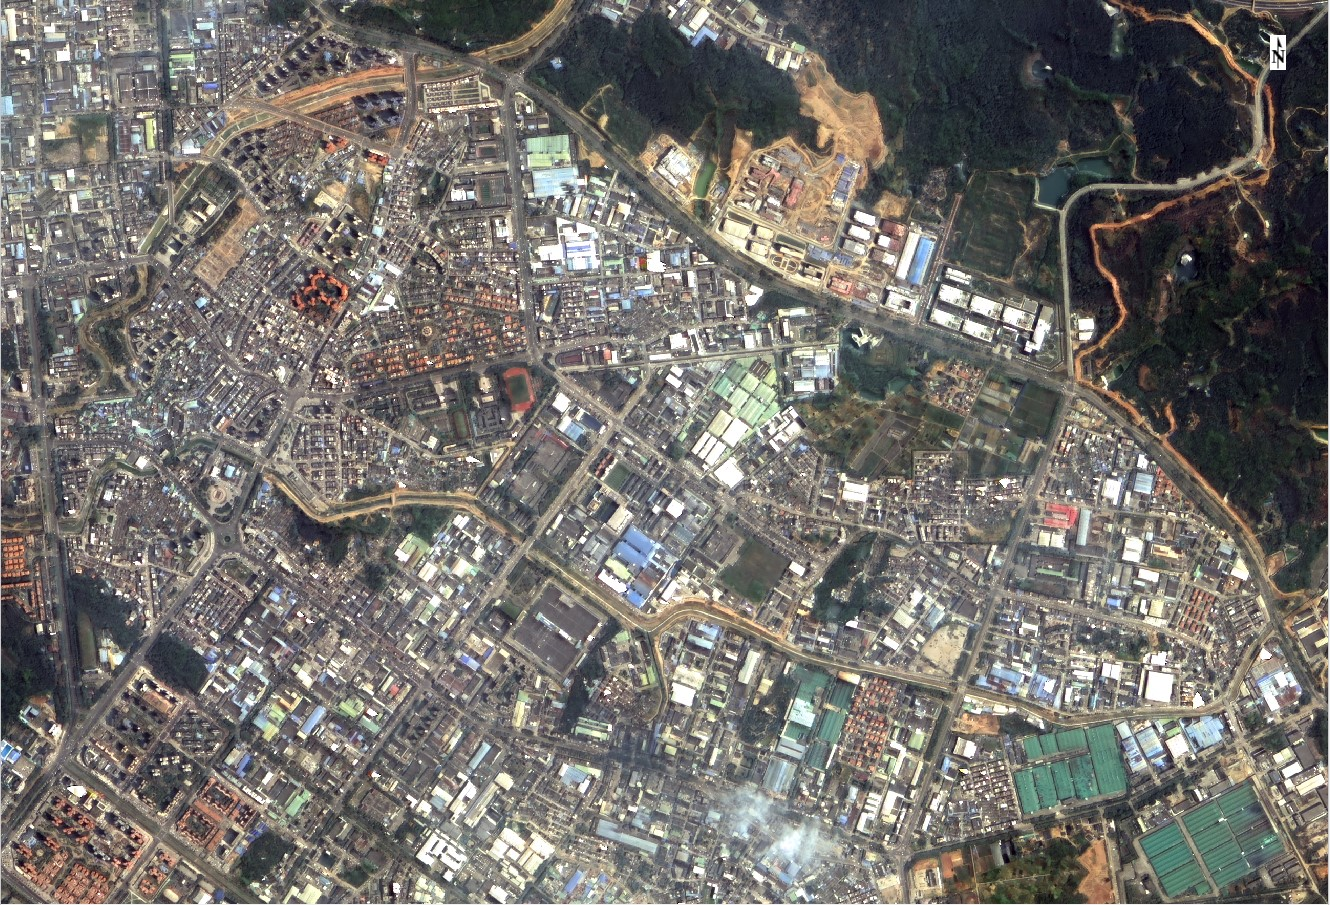
\includegraphics[height=20em]{pic/res01_02.jpg}}
    \caption{影像精匹配结果}
    \label{fig:0217}
\end{figure}